% Copyright 2007 by Till Tantau
%
% This file may be distributed and/or modified
%
% 1. under the LaTeX Project Public License and/or
% 2. under the GNU Public License.
%
% See the file doc/licenses/LICENSE for more details.



\documentclass{beamer}

%
% DO NOT USE THIS FILE AS A TEMPLATE FOR YOUR OWN TALKS�!!
% bleh :D
% Use a file in the directory solutions instead.
% They are much better suited.
%


% Setup appearance:

% \usetheme{Darmstadt}
% \usetheme{Lleida}
 \usetheme{Frankfurt}
% \usetheme{Singapore}

\usefonttheme[onlylarge]{structurebold}
\setbeamerfont*{frametitle}{size=\normalsize,series=\bfseries}
%\setbeamertemplate{navigation symbols}{}


% Standard packages

\usepackage[english]{babel}
\usepackage[latin1]{inputenc}
\usepackage{times}
\usepackage[T1]{fontenc}

% Setup TikZ

\usepackage{tikz}
\usetikzlibrary{arrows}
\tikzstyle{block}=[draw opacity=0.7,line width=1.4cm]


% Setup pygments
\usepackage{fancyvrb}
\usepackage{color}
\newcommand\PYZat{@}
\newcommand\PYZlb{[}
\newcommand\PYZrb{]}
\newcommand\PYbh[1]{\textcolor[rgb]{0.00,0.50,0.00}{\textbf{#1}}}
\newcommand\PYbg[1]{\textcolor[rgb]{0.73,0.40,0.53}{\textbf{#1}}}
\newcommand\PYbf[1]{\textcolor[rgb]{0.82,0.25,0.23}{\textbf{#1}}}
\newcommand\PYbe[1]{\textcolor[rgb]{0.40,0.40,0.40}{#1}}         
\newcommand\PYbd[1]{\textcolor[rgb]{0.73,0.13,0.13}{#1}}         
\newcommand\PYbc[1]{\textcolor[rgb]{0.00,0.50,0.00}{\textbf{#1}}}
\newcommand\PYbb[1]{\textcolor[rgb]{0.00,0.50,0.00}{#1}}         
\newcommand\PYba[1]{\textcolor[rgb]{0.00,0.00,0.50}{\textbf{#1}}}
\newcommand\PYaJ[1]{\textcolor[rgb]{0.69,0.00,0.25}{#1}}         
\newcommand\PYaK[1]{\textcolor[rgb]{0.73,0.13,0.13}{#1}}         
\newcommand\PYaH[1]{\textcolor[rgb]{0.50,0.00,0.50}{\textbf{#1}}}
\newcommand\PYaI[1]{\fcolorbox[rgb]{1.00,0.00,0.00}{1,1,1}{#1}}  
\newcommand\PYaN[1]{\textcolor[rgb]{0.74,0.48,0.00}{#1}}         
\newcommand\PYaO[1]{\textcolor[rgb]{0.00,0.00,1.00}{\textbf{#1}}}
\newcommand\PYaL[1]{\textcolor[rgb]{0.00,0.00,1.00}{#1}}         
\newcommand\PYaM[1]{\textcolor[rgb]{0.73,0.73,0.73}{#1}}         
\newcommand\PYaB[1]{\textcolor[rgb]{0.73,0.13,0.13}{#1}}         
\newcommand\PYaC[1]{\textcolor[rgb]{0.67,0.13,1.00}{#1}}         
\newcommand\PYaA[1]{\textcolor[rgb]{0.00,0.50,0.00}{#1}}         
\newcommand\PYaF[1]{\textcolor[rgb]{0.63,0.00,0.00}{#1}}         
\newcommand\PYaG[1]{\textcolor[rgb]{1.00,0.00,0.00}{#1}}         
\newcommand\PYaD[1]{\textcolor[rgb]{0.00,0.50,0.00}{\textbf{#1}}}
\newcommand\PYaE[1]{\textcolor[rgb]{0.25,0.50,0.50}{\textit{#1}}}
\newcommand\PYaZ[1]{\textcolor[rgb]{0.00,0.50,0.00}{\textbf{#1}}}
\newcommand\PYaX[1]{\textcolor[rgb]{0.00,0.50,0.00}{#1}}         
\newcommand\PYaY[1]{\textcolor[rgb]{0.73,0.13,0.13}{#1}}         
\newcommand\PYaR[1]{\textcolor[rgb]{0.40,0.40,0.40}{#1}}         
\newcommand\PYaS[1]{\textcolor[rgb]{0.10,0.09,0.49}{#1}}         
\newcommand\PYaP[1]{\textcolor[rgb]{0.00,0.00,0.50}{\textbf{#1}}}
\newcommand\PYaQ[1]{\textcolor[rgb]{0.49,0.56,0.16}{#1}}         
\newcommand\PYaV[1]{\textcolor[rgb]{0.00,0.00,1.00}{\textbf{#1}}}
\newcommand\PYaW[1]{\textcolor[rgb]{0.73,0.13,0.13}{#1}}         
\newcommand\PYaT[1]{\textcolor[rgb]{0.40,0.40,0.40}{#1}}         
\newcommand\PYaU[1]{\textcolor[rgb]{0.25,0.50,0.50}{\textit{#1}}}
\newcommand\PYaj[1]{\textcolor[rgb]{0.00,0.50,0.00}{#1}}         
\newcommand\PYak[1]{\textcolor[rgb]{0.73,0.40,0.53}{#1}}         
\newcommand\PYah[1]{\textcolor[rgb]{0.63,0.63,0.00}{#1}}         
\newcommand\PYai[1]{\textcolor[rgb]{0.10,0.09,0.49}{#1}}         
\newcommand\PYan[1]{\textcolor[rgb]{0.40,0.40,0.40}{#1}}         
\newcommand\PYao[1]{\textcolor[rgb]{0.73,0.40,0.13}{\textbf{#1}}}
\newcommand\PYal[1]{\textcolor[rgb]{0.25,0.50,0.50}{\textit{#1}}}
\newcommand\PYam[1]{\textbf{#1}}                                 
\newcommand\PYab[1]{\textit{#1}}                                 
\newcommand\PYac[1]{\textcolor[rgb]{0.73,0.13,0.13}{#1}}         
\newcommand\PYaa[1]{\textcolor[rgb]{0.50,0.50,0.50}{#1}}         
\newcommand\PYaf[1]{\textcolor[rgb]{0.25,0.50,0.50}{\textit{#1}}}
\newcommand\PYag[1]{\textcolor[rgb]{0.40,0.40,0.40}{#1}}         
\newcommand\PYad[1]{\textcolor[rgb]{0.00,0.25,0.82}{#1}}         
\newcommand\PYae[1]{\textcolor[rgb]{0.40,0.40,0.40}{#1}}         
\newcommand\PYaz[1]{\textcolor[rgb]{0.00,0.63,0.00}{#1}}         
\newcommand\PYax[1]{\textcolor[rgb]{0.60,0.60,0.60}{\textbf{#1}}}
\newcommand\PYay[1]{\textcolor[rgb]{0.00,0.50,0.00}{\textbf{#1}}}
\newcommand\PYar[1]{\textcolor[rgb]{0.10,0.09,0.49}{#1}}         
\newcommand\PYas[1]{\textcolor[rgb]{0.73,0.13,0.13}{\textit{#1}}}
\newcommand\PYap[1]{\textcolor[rgb]{0.00,0.50,0.00}{\textbf{#1}}}
\newcommand\PYaq[1]{\textcolor[rgb]{0.53,0.00,0.00}{#1}}         
\newcommand\PYav[1]{\textcolor[rgb]{0.67,0.13,1.00}{\textbf{#1}}}
\newcommand\PYaw[1]{\textcolor[rgb]{0.40,0.40,0.40}{#1}}         
\newcommand\PYat[1]{\textcolor[rgb]{0.10,0.09,0.49}{#1}}         
\newcommand\PYau[1]{\textcolor[rgb]{0.10,0.09,0.49}{#1}}    
%pygmentize -f latex hello.py
%\begin{frame}[fragile]
%\begin{Verbatim}[commandchars=@\[\]]
%@PYaD[#!/usr/bin/env python]
%@PYay[print] @PYad["]@PYad[hello]@PYad["]
%\end{Verbatim}

% Author, Title, etc.

\title[Experimentation with python - why not do it the FOSS way?] 
{%
  \textbf{Experimentation with python} \\ \textit{Why not do it the FOSS way?}%
}

\author[Suryajith, Praneeth]
{
  Suryajith Chillara\inst{1} \and
  Praneeth Bodduluri\inst{1}
}

\institute[IIT Kanpur]
{
  \inst{1}%
  Indian Institute of Technology, Kanpur
}

\date[SciPy.in 2009]
{SciPy India Conference, 2009}



% The main document

\begin{document}

\begin{frame}
  \titlepage
\end{frame}

\begin{frame}{Outline}
  \tableofcontents
\end{frame}


\section{Introduction}


\begin{frame}[fragile]{Current state of instrumentation software} 
\begin{block}{}
\begin{itemize}
 \item LabVIEW $\implies$ Proprietary
\uncover<2->{
 \item C $\implies$ Write some code and debug forever
 \uncover<3>{\item Python $\implies$ What is python?
}}
\end{itemize}
\end{block}
\end{frame}

\section{LabVIEW}

\subsection{Why is it popular? }
\begin{frame}{LabVIEW: Why is it popular?}
\begin{block}{}
\begin{itemize}
 \item Graphical programming environment \\$\implies$ Drag Drop , Click Connect
 \item Idea of low level communication protocols \\$\implies$ Minimal $\implies$ Good / bad?
 \item A double clickable installer for almost all hardware [$\ddot\smile$]
\end{itemize}
\end{block}
\end{frame}
\begin{frame}{LabVIEW: Why is it popular?}
   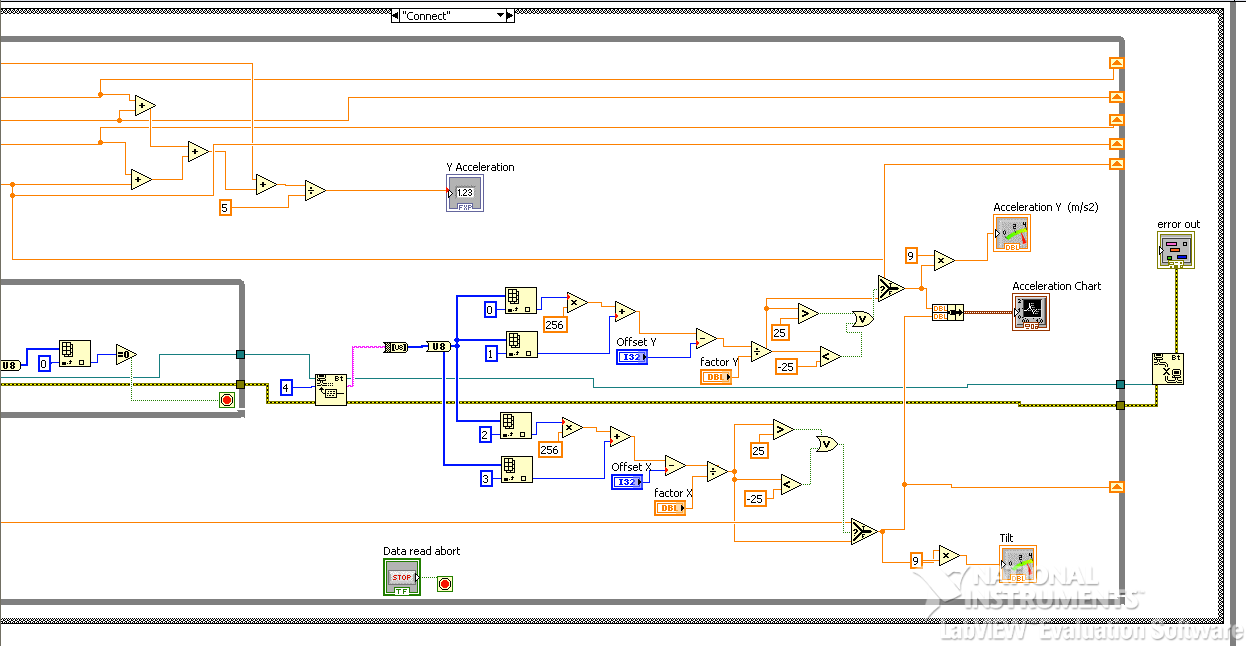
\includegraphics[width=115mm,height=70mm]{labview.png}
\end{frame}

\subsection{So whats bad about it?}
\begin{frame}{LabVIEW: So whats bad about it?}
 \begin{block}{}
\begin{itemize}
	\item The LabVIEW(TM) Academic Premium Suite \\Cost ( single user ) $\implies$ INR 111,600.00
	 \uncover<2->{ \item  Building a stand-alone application requires a separate purchase if using the Base Package or Full Development System
	\uncover<3>{ \item Compiled executables produced by LabVIEW are not truly standalone in that they also require that the LabVIEW run-time engine be installed on any target computer on which users run the application.}}
\end{itemize}
\end{block}
\end{frame}

\begin{frame}{LabVIEW: So whats bad about it?}
 \begin{block}{}
  \begin{itemize}
   \item Support for non Windows platforms is poor.
   \uncover<2->{\item While it is easy to produce seemingly parallel code, it is difficult for beginners to control this at a fine-grained level making multi-interface systems unwieldy and unreliable. 
	\uncover<3>{\item The detailed complexity of such systems is often hidden and inaccessible or obfuscated by the top-level design, making procedural events across devices difficult to manage.
	}}
  \end{itemize}

 \end{block}
\end{frame}

\section{Are there any Open Source alternatives?}
\begin{frame}{Are there any Open Source alternatives?}
 \begin{block}{}
  \begin{itemize}
 \item None that match the graphical programming environment of LabVIEW
 \uncover<2>{\item  Python $\implies$ close enough with its simplistic approach.}
\end{itemize}

 \end{block}

\end{frame}

\section{Why/How do we do it with Python?}
\begin{frame}{Why/How do we do it with Python?}
 \begin{block}{}
  \begin{itemize}
   \item Most of the devices run with either a GPIB , Serial or TCP/IP
   \uncover<2->{\item Scripting environment to enable quick debugging + SWIG incase you itch for those extra optimizations
     \uncover<3->{\item Can generate standalone cross platform applications with py2exe or py2dmg (We dont need one for linux [$\ddot\smile$] )
       \uncover<4>{\item Follows the usual programming paradigms \begin{center}  $\implies$ Making it simpler to get hooked on to, if one lets go of the initial fear of foreign languages.\end{center}}}}
  \end{itemize}
 \end{block}
\end{frame}
\begin{frame}[fragile]{Why/How do we do it with Python?}
\begin{itemize}
 \item Packages like PySerial and PyVISA that enable easy connectivity with your instruments.
\end{itemize}
\underline{A PySerial example:}
\begin{Verbatim}[commandchars=@\[\]]                                               
@PYbc[import] @PYaV[serial],@PYaV[time],@PYaV[csv]                       
@PYaE[#open the serial port]                                                       
ser @PYbe[=] serial@PYbe[.]Serial(@PYaB[']@PYaB[COM4]@PYaB['], @PYaw[19200], timeout@PYbe[=]@PYaw[1])
@PYaE[#set input1 to counter A]                                                                      
ser@PYbe[.]write(@PYaB["]@PYaB[CI 0,1]@PYaB["])                                                      
ser@PYbe[.]write(@PYaB[']@PYao[\n]@PYaB['])                                                          
@PYaE[# set the sampling time]                                                                       
@PYaE[# -> 1E4(1 ms) Denotes the no of 10MHz cycles]                                                 
ser@PYbe[.]write(@PYaB["]@PYaB[CP2,1E4]@PYaB["])                                                     
ser@PYbe[.]write(@PYaB[']@PYao[\n]@PYaB['])                                                          
@PYaE[# set count mode to A,B]                                                                       
ser@PYbe[.]write(@PYaB["]@PYaB[CM 0]@PYaB["])                                                        
\end{Verbatim}
\end{frame}
\begin{frame}[fragile]{Why/How do we do it with Python?}
\begin{Verbatim}[commandchars=@\[\]]                                               
ser@PYbe[.]write(@PYaB[']@PYao[\n]@PYaB['])                                                          
@PYaE[# set discriminator A to fall mode]                                                            
ser@PYbe[.]write(@PYaB["]@PYaB[DS 1,1]@PYaB["])                                                      
ser@PYbe[.]write(@PYaB[']@PYao[\n]@PYaB['])                                                          
@PYaE[# set discriminator level]                                                                     
ser@PYbe[.]write(@PYaB["]@PYaB[DL 0,-0.0036]@PYaB["])                                                
ser@PYbe[.]write(@PYaB[']@PYao[\n]@PYaB['])                                                          
@PYay[print] @PYaB[']@PYaB[Completed]@PYaB[']                                                        
@PYay[print] @PYaB[']@PYaB[0]@PYaB[%]@PYaB['], 
@PYaE[# Open file in append mode]                                                                    
Han @PYbe[=] @PYaX[open](@PYaB["]@PYaB[data.csv]@PYaB["],@PYaB["]@PYaB[a]@PYaB["])                   
FILE @PYbe[=] csv@PYbe[.]writer(Han)
\end{Verbatim}
\end{frame}


\begin{frame}[fragile]{Why/How do we do it with Python?}
\begin{Verbatim}[commandchars=@\[\]]                                               
@PYaE[#100 samples]
@PYay[for] i @PYav[in] @PYaX[range](@PYaw[1],@PYaw[100]):
    ser@PYbe[.]write(@PYaB["]@PYaB[CS]@PYaB["])
    ser@PYbe[.]write(@PYaB[']@PYao[\n]@PYaB['])
    time@PYbe[.]sleep(@PYbe[.]@PYaw[5])
    ser@PYbe[.]write(@PYaB["]@PYaB[QA1]@PYaB["])
    ser@PYbe[.]write(@PYaB[']@PYao[\n]@PYaB['])
@PYaE[# The instrument gives 3 bytes]
    name @PYbe[=] ser@PYbe[.]read(@PYaw[3])
    FILE@PYbe[.]writerow(@PYZlb[]@PYaX[str](name)@PYZrb[])
    ser@PYbe[.]write(@PYaB["]@PYaB[CR]@PYaB["])
    ser@PYbe[.]write(@PYaB[']@PYao[\n]@PYaB['])
    @PYay[print] @PYaB[']@PYao[\b]@PYao[\b]@PYao[\b]@PYao[\b]@PYaB[']@PYbe[+]@PYaX[str](i)@PYbe[+]@PYaB[']@PYaB[%]@PYaB[']
ser@PYbe[.]close()
Han@PYbe[.]close()
\end{Verbatim}
\end{frame}
\begin{frame}[fragile]{Note}
  \begin{block}{}
  \begin{itemize}
  	\item Approximate RAM usage 
	\begin{itemize}
		\item Labview : 300 MB 
		\item Python \ \ :\ \ \  20 MB
	\end{itemize}
  \end{itemize}
\end{block}
\underline{A PyVISA example:}
\begin{Verbatim}[commandchars=@\[\]]
@PYbc[from] @PYaV[visa] @PYbc[import] instrument

myinstrument @PYbe[=] instrument(@PYaB["]@PYaB[GPIB::12]@PYaB["])
myinstrument@PYbe[.]write(@PYaB["]@PYaB[*rst; status:preset; *cls]@PYaB["])
myinstrument@PYbe[.]ask(@PYaB["]@PYaB[status:measurement?]@PYaB["])
\end{Verbatim}
\end{frame}

\begin{frame}{Why/How do we do it with Python?}
    
\includegraphics[width=119mm,height=60mm]{modules.png}
\end{frame}


\section*{Summary}
\begin{frame}{}

\textbf{\begin{center}
         Questions?
        \end{center}}
\end{frame}
\end{document}


